\section{Extension to Full Macro}
Large scale full macro extension involves Skill Script schematic circuit design automation, scaling it up to arbitrary size, because it is not practical and almost impossible to have hand drawn circuit at large scale. 4 version iterations were undergone to overcome design challenges (See Challenges section) and adding new features. All testing wise are automated. Generally, $V_{\text{in}}$ are randomly generated. Each of the $n$ random $V_{\text{in}}$ has a value $0V\geq V_{\text{in}} \geq \frac{V_{\text{sat}}}{n}$ so that sum of all these values will not exceed $V_{\text{sat}}$ and get clipped. Weights $w$ are randomly generated and the output of all neuron are monitored and compared against the ideal values through finding the mean and standard deviation of all neurons.
\subsection{$\text{1}^{\text{st}}$ version} % simple
\begin{figure}[H]
	\centering
	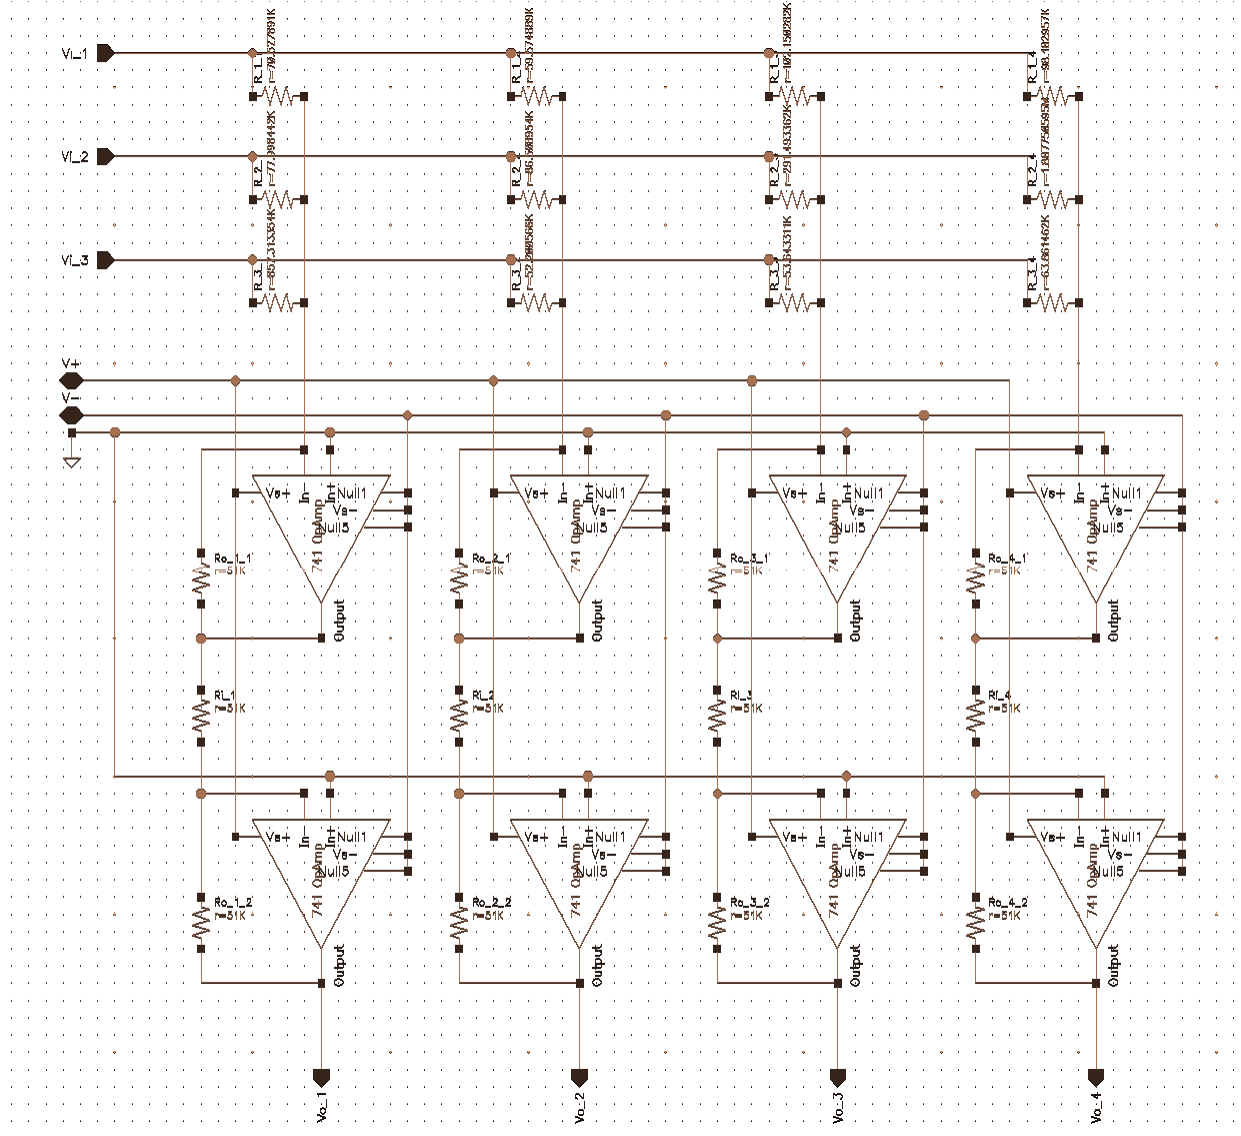
\includegraphics[scale=0.5]{version1.png}
	\caption{4 by 3 generated summing neuron design implemented in Cadence}
	\label{fig:ver1}
\end{figure}
Figure \ref{fig:ver1} is simply a scaling up of Figure \ref{fig:singleneuron}. Since the weight is between $0\geq w \geq1$, the corresponding resistance is $\infty \leq R \leq1$, but for practical consideration, $\infty$ resistance is limited at $\frac{1}{0.001}\Omega=1000\Omega$ which should suffice when compared to high weight ($w=1$) or low resistance of ($R=1\Omega$). 
\begin{figure}[H]
	\centering
	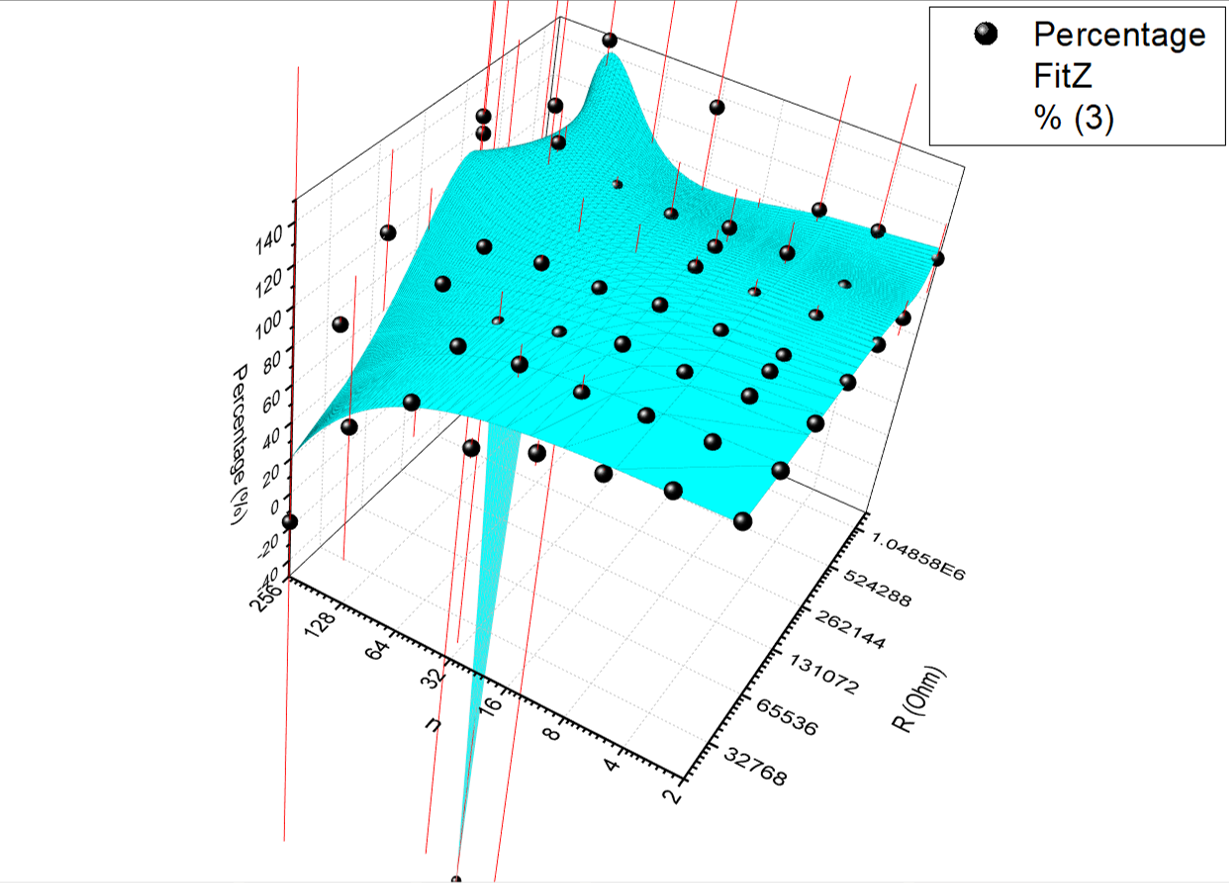
\includegraphics[scale=0.5]{singlerfadj.png}
	\caption{Optimal $R_F$ value determination for large scale circuit (for parameters data, see Appendix Table \ref{tbl:singlerfparam})}
	\label{fig:rfsinglescale}
\end{figure}
From Equation \ref{eq:finalsimplified}, the full equation for a single neuron output is:
$$V_{\text{out}} =-\frac{R_{F2}}{R_{\text{out}'}}\left( -R_{F1}\left( \frac{V_1}{R_1\left| R_F\right| } + \frac{V_2}{R_2\left| R_F\right| } + \frac{V_3}{R_3\left| R_F\right| }+...+\frac{V_n}{R_n\left| R_F\right| }\right) \right) $$
We could have set $R_{\text{out}'}$, $R_{F2}$, $R_{F1}$ to $1\Omega$ but this is not possible due to practical challenges (see challenges section), so an $\left| R_F\right|$ magnitude is add to every $R_n$ such that:
\begin{equation}
\label{cond:rf}
R=\left|R_{\text{out}'}\right|=\left|R_{F2}\right|=\left|R_{F1}\right|=\left| R_F\right|
\end{equation} to maintain the same Equation \ref{eq:final} and thus the physical $R_{\text{phy}}=R_n\left| R_F\right|$.

In a matrix form for $m$ neuron outputs, we have:
$$\begin{bmatrix}
V_{\text{o1}} \\
V_{\text{o2}} \\
\vdots \\
V_{\text{om}}
\end{bmatrix}=-R_{F2}
\begin{bmatrix} 
\frac{1}{R_{\text{out}'}} &  &  \\
& \ddots & \\
&        & \frac{1}{R_{\text{out}'}}
\end{bmatrix}
\left[-R_{F1}\begin{bmatrix}
\frac{1}{R_{11}\left| R_F\right|} & \frac{1}{R_{21}\left| R_F\right|} & \cdots & \frac{1}{R_{n1}\left| R_F\right|} \\
\frac{1}{R_{12}\left| R_F\right|} & \frac{1}{R_{22}\left| R_F\right|} & \cdots & \frac{1}{R_{n2}\left| R_F\right|} \\
\vdots & \vdots & & \vdots \\
\frac{1}{R_{1m}\left| R_F\right|} & \frac{1}{R_{2m}\left| R_F\right|} & \cdots & \frac{1}{R_{nm}\left| R_F\right|}
\end{bmatrix}\right] 
\begin{bmatrix}
V_{\text{i1}} \\
V_{\text{i2}} \\
\vdots \\
V_{\text{in}}
\end{bmatrix}$$

In Figure \ref{fig:rfsinglescale}, average percentage of measured $V_{\text{out}}$ value is plotted against $n$ number of input $V_{\text{in}}$ and magnitude $R$. When $n$ and $R$ are small, percentage average is predictable, as we can see the surface plot fit nicely, but towards the extreme ends, the values get unpredictable as the errors got out of hand (see Challenges section), as the limit of scaling is reached.
\subsection{$\text{2}^{\text{nd}}$ version} % nmos or pmos
\begin{figure}[H]
	\centering
	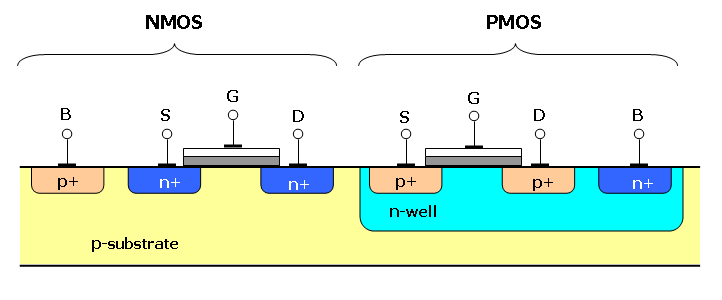
\includegraphics[scale=0.5]{cmos.png}
	\caption{Complementary metal oxide semiconductor (CMOS)}
	\label{fig:cmos}
\end{figure}
Complementary metal oxide semiconductor (CMOS) is involved as we are looking for voltage-controlled switches to isolate and program physical resistances $R_{phy}$. We assume the resistances are programmable when they are isolated and extreme voltages (outside of normal operating range) are applied and caused a physical lasting change in their resistances. There are a few similar types of resistive memory pertaining to our assumption here (conductive-bridging RAM (CBRAM), and phase-change memory, etc.) but they are out of our scope of discussion and we will not explore them here.

In Figure \ref{fig:cmos}, we have n channel MOSFET (NMOS) and p channel MOSFET (PMOS). These 2 MOSFETs, together are known as CMOS. PMOS sit in n-well, with p-type diffusion on an n-type substrate.
For PMOS to operate, source S voltage $V_s$ is held at high, gate G voltage $V_g$ lower than $V_s$, and drain voltage at the lowest among all. When $V_g=V_s$, PMOS does not operate. However, when we lower $V_g$ to a point where $V_{gs} \leq V_t$ ($V_{gs}$ being negative and $V_t$ is the threshold voltage), PMOS switches on (p channel is formed from source to drain and current flow with holes as the majority carrier).

Similarly and yet being different, NMOS operation involves source S voltage $V_s$ held at low, gate G voltage $V_g$ higher than $V_s$, and drain voltage at the highest among all. When $V_g=V_s$, NMOS is at the cut off region. However, when we increase $V_g$ to a point where $V_{gs} \geq V_t$, NMOS switches on (n channel is formed from source to drain and current flow with electrons as the majority carrier).

Both NMOS and PMOS body terminal voltage are tied to their source voltage to maintain their $V_t$.
\begin{figure}[H]
	\centering
	\def\svgwidth{100pt}
	\input{inverter.pdf_tex}
	\caption{Complementary metal oxide semiconductor (CMOS) inverter with PMOS on top and NMOS below}
\end{figure}
A simplest device by PMOS and NMOS is the inverter. PMOS is marked with a hollow circle above whereas NMOS is situated below. A is the input and Q is the output. $V_{\text{dd}}$ is held at high voltage and $V_{\text{ss}}$ is held at low voltage. When input A is high ($V_{\text{dd}}$),  PMOS is off and NMOS is on, hence Q is low ($V_{\text{ss}}$). Conversely, if input A is low ($V_{\text{ss}}$),  NMOS is off and PMOS is on, hence Q is high ($V_{\text{dd}}$). Hence, we are assuming ideal short circuit on and off behaviour of CMOS.

However, practically, PMOS and NMOS have finite resistance. Their ADE measured on resistance is at $k\Omega$ range, and their off resistance is at $G\Omega$ range. For domain wall based MRAM resistance range of ($1k\Omega$ to $3k\Omega$), we have trouble differentiating the MRAM resistance and CMOS on resistance, thus they affects our result negatively.
\begin{table}[H]
	\centering
	\begin{tabular}[t]{ccc}
		\hline
		MOSFET Type & On Resistance ($\Omega$) & Off Resistance ($\Omega$)\\
		\hline
		\hline
		pch\_18 & 3.43k & 1.316G\\
		pch & 2.32k & 24G\\
		nch & 1.2k & 3.44G\\
		nch\_18 &  1.5k & 785.8M\\            
		\hline
	\end{tabular}
	\caption{Table of MOSFET type supplied by process design kit (PDK) from foundries and their on/off resistance}
\end{table}
PMOS and NMOS based design were tested as shown in Figure \ref{fig:pmosscaled} (only showing PMOS). Circuit execution wise is the same as that of the $\text{1}^{\text{st}}$ version. The only difference is the circuit weights are made programmable through isolation.

In MOSFET execution mode, all MOSFETs are set to on, such that all the programmable resistors (weights) array is connected to the summing opamps neuron. In programming mode, resistors are programmed row by row because we have $V_{\text{en\_n}}$, wires routed to the MOSFETs in series with the resistors row by row. MOSFETs of the current row of interest are all turned on, while the remaining are turned off, thus isolating all other rows from the programming action. $V_{\text{in}}$ or $V_{\text{i\_n}}$ pins on the left of the row of interest is set as reference voltage whereas $V_{\text{in,set}}$ or $V_{\text{is\_n}}$ (from the top) of the individual resistances on that row is set individually.

NMOS performance is better than PMOS, but not by a wide margin. With $n = 10$ number of inputs and $m = 20$ number of neuron outputs and $R=50k\Omega$ (Condition \ref{cond:rf}), NMOS circuit performance (average measured percentage in relation to ideal) vs that of PMOS is $80.3\pm3.0\%
$ vs $67.7\pm4.0\%$. One reason is NMOS majority charge carriers (electrons) have higher mobility as compared to that (holes) of PMOS.
\begin{figure}[H]
	\centering
	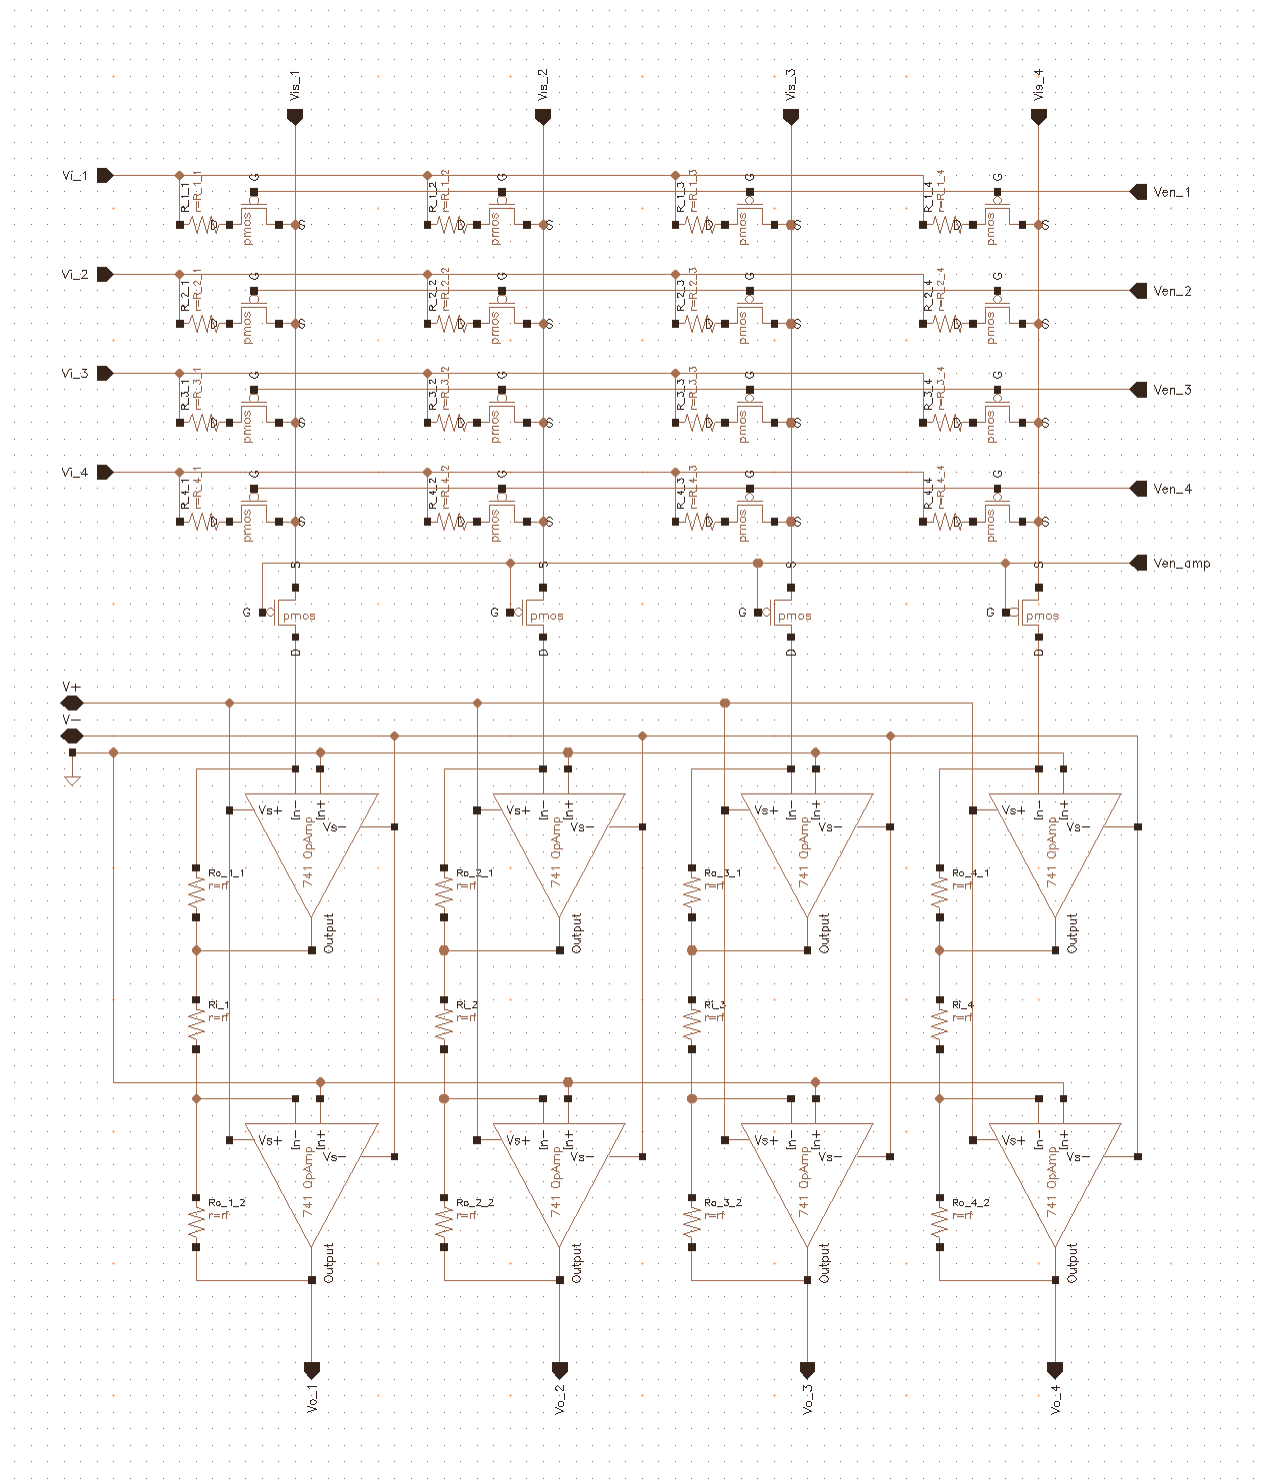
\includegraphics[scale=0.5]{version2.png}
	\caption{4 by 4 generated summing neuron with pmos design implemented in Cadence}
	\label{fig:pmosscaled}
\end{figure}
\subsection{$\text{3}^{\text{rd}}$ and $\text{4}^{\text{th}}$ versions}
A proposal has been put forward by co-supervisor about mimicking simplified MRAM resistance property (with limited 8 step $1k\Omega-3k\Omega$), while preserving the actual weight range (also see Case Study section for additional detailed explanation). Resistance and weight relationship in Table \ref{fig:rnw} is used when designing the $\text{3}^{\text{rd}}$ and $\text{4}^{\text{th}}$ versions neuromorphic circuit. The physical resistance $r_{p}$ is what actually went into the circuit and they represent compressed weight $w_{c}$, additional circuit are added to restore the original weight representation (decompressed weight $w_{d}$).
\begin{table}[H]
	\centering
	\begin{tabular}[t]{ccccc}
		\hline
		Index & Physical Resistance $r_{p}$ ($\Omega$) & Resistance $r$ ($\Omega$) & Compressed Weight $w_{c}$ & Decompressed Weight $w_{d}$\\
		\hline
		\hline
		0 & 1000 & 1.0 & 1.0 & 1.0\\
		1 & 1250 & 1.25 & 0.8 & 0.7\\
		2 & 1500 & 1.5 & 0.6667 & 0.4999\\
		3 & 1750 &  1.75 & 0.5714 & 0.3571\\
		4 & 2000 & 2.0 & 0.5 & 0.25\\
		5 & 2250 & 2.25 & 0.4444 & 0.1667\\
		6 & 2500 & 2.5 & 0.4 & 0.1000\\
		7 & 2750 & 2.75 & 0.3636 & 0.0454\\
		8 & 3000 & 3.0 & 0.3333 & 0\\            
		\hline
	\end{tabular}
	\caption{Table of resistances and weights}
	\label{fig:rnw}
\end{table}
Here, we set
$w_{c,0} = 1$ and $r_{0} = 1/w_{c,0}$, where the subscript number after comma is the index.\\
Hence,
$$r_i = \frac{r_{p,i}}{1000}$$
\begin{equation}
\label{eq:rwmap}
w_{c,i} = 1/r_i
\end{equation}
\begin{equation}
\label{eq:wmap}
w_{d,i} = \frac{w_{c,i}-w_{c,8}}{w_{c,0}-w_{c,8}}
\end{equation}

The decompression mechanism for circuit implementation is derived as follows:
\begin{quote}
	We need to achieve:
	$$V_{\text{out}}=w_{d,i_1}V_1+w_{d,i_2}V_2+...$$
	and we know from:
	\begin{enumerate}
		\item Equation \ref{eq:rwmap}:\\ Compressed weights $w_{c,i}$ are directly related to resistance $r$ and thus the physical resistances $r_p$.
		\item Equation \ref{eq:wmap}:\\
		The relationship between compressed weight $w_{c,1}$ and decompressed weight $w_{d,1}$.
	\end{enumerate}
	Hence,
	$$V_{\text{out}}=\frac{w_{c,i_1}-w_{c,8}}{w_{c,0}-w_{c,8}}V_1+\frac{w_{c,i_2}-w_{c,8}}{w_{c,0}-w_{c,8}}V_2+...$$
	and
	$$V_{\text{out}}=\frac{\frac{1}{r_1}-w_{c,8}}{w_{c,0}-w_{c,8}}V_1+\frac{\frac{1}{r_2}-w_{c,8}}{w_{c,0}-w_{c,8}}V_2+...$$
	and finally for a single neuron output:
	\begin{equation}
	\label{eq:final34compdecomp}
	V_{\text{out}}=\frac{1}{w_{c,0}-w_{c,8}}\left( \left(\frac{1}{r_1}V_1+\frac{1}{r_2}V_2+... \right)-\left(w_{c,8}V_1+w_{c,8}V_2+... \right)\right)
	\end{equation}
	for $m$ neuron outputs:
	\begin{equation}
	\label{eq:finalncompdecomp}
	\begin{bmatrix}
	V_{\text{o1}} \\
	V_{\text{o2}} \\
	\vdots \\
	V_{\text{on}}
	\end{bmatrix}=\frac{1}{w_{c,0}-w_{c,8}}
	\left[ 
	\begin{bmatrix}
	\frac{1}{R_{11}} & \frac{1}{R_{21}} & \cdots & \frac{1}{R_{n1}} \\
	\frac{1}{R_{12}} & \frac{1}{R_{22}} & \cdots & \frac{1}{R_{n2}} \\
	\vdots & \vdots & & \vdots \\
	\frac{1}{R_{1m}} & \frac{1}{R_{2m}} & \cdots & \frac{1}{R_{nm}}
	\end{bmatrix}
	\begin{bmatrix}
	V_{\text{i1}} \\
	V_{\text{i2}} \\
	\vdots \\
	V_{\text{in}}
	\end{bmatrix}
	-\begin{bmatrix}
	w_{c,8} &  \cdots & w_{c,8} \\
	\vdots &  & \vdots \\
	w_{c,8} & \cdots & w_{c,8}
	\end{bmatrix}
	\begin{bmatrix}
	V_{\text{i1}} \\
	V_{\text{i2}} \\
	\vdots \\
	V_{\text{in}}
	\end{bmatrix}
	\right] 
	\end{equation}
\end{quote}
The term $\left(\frac{1}{r_1}V_1+\frac{1}{r_2}V_2+... \right)$ can be implemented by normal summation using the $\text{1}^{\text{st}}$ row opamp, which results in $-\left(\frac{1}{r_1}V_1+\frac{1}{r_2}V_2+... \right)$. By going through a opamp again with a fixed scale factor $\frac{1}{w_{c,0}-w_{c,8}}$, the term $\left(w_{c,8}V_1+w_{c,8}V_2+... \right)$ can be sum up separately, together with the previous term, and an inverting sign, yields Equation \ref{eq:final34compdecomp} as needed.

Table \ref{fig:rnw} was examined further by manipulating the scale factor $s$ of compressed weight i.e. $\left[ \frac{1}{3s},\frac{1}{s}\right]$, with the boundary plotted in Figure \ref{fig:scaledr}. When $s=1$, we obtain $w_c$ boundary $w_{\text{c,0}}=1.0$ and $w_{\text{c,8}}=0.3333$ same as that of Table \ref{fig:rnw}. As scale factor $s$ increases, the boundary tends towards 0 and compressed weight can no longer be represented faithfully. This figure is mainly used in our case study weight processing functions and their influence on our result (see more in that section). Figure \ref{fig:rwrel} shows clearly the inverse relation between compressed weight $w_c$ and resistance $r$. Ideally, we would want uniform steps in $w$. However, due to this inverse relationship, what initially uniform in terms of $r$ results in non uniformity of $w$. This non uniformity of $w$ can distort our represented compressed weight and affect our result negatively.
\begin{figure}[H]
	\centering
	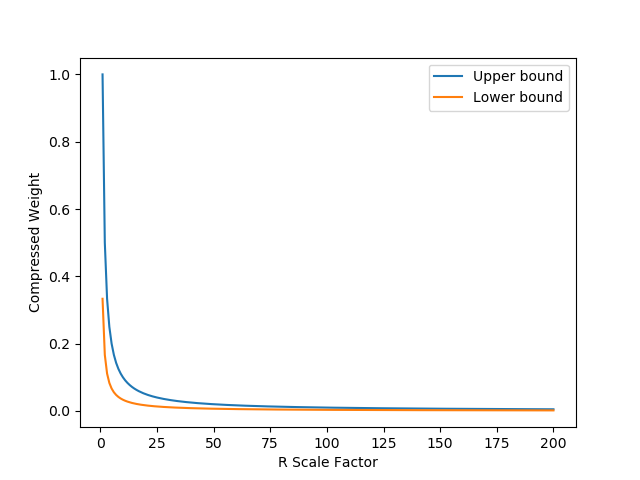
\includegraphics[scale=0.6]{scaledr.png}
	\caption{Graph of range of values for compressed weight $w_c$ with scaled R}
	\label{fig:scaledr}
\end{figure}
\begin{figure}[H]
	\centering
	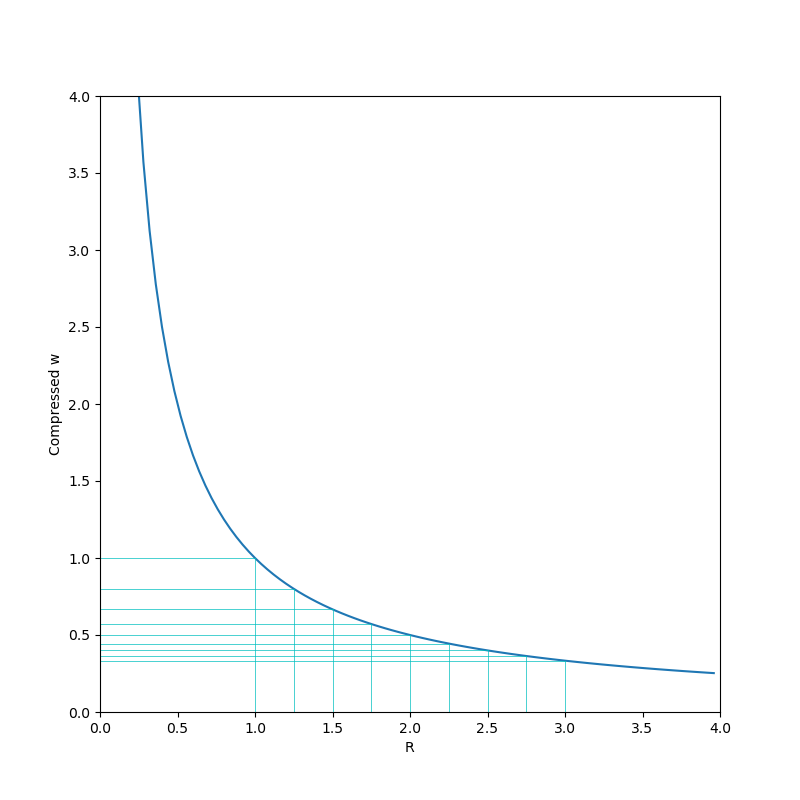
\includegraphics[scale=0.7]{rw.png}
	\caption{Graph of relationship between uniform R and non-uniform compressed weight}
	\label{fig:rwrel}
\end{figure}
\subsubsection{$\text{3}^{\text{rd}}$ version} % no nmos or pmos, extra circuit
A design put forward by D. Kaushik et al \cite{kaushik} showed that programming 8 bit DW MRAM doesn't require isolation because read and write operation in DW MRAM are independent of each other. Hence, the problem encountered in $\text{2}^{\text{nd}}$ version where MOSFET on resistance in the range of MRAM resistance range can be side stepped. Hence, all MOSFET are removed.
\begin{figure}[H]
	\centering
	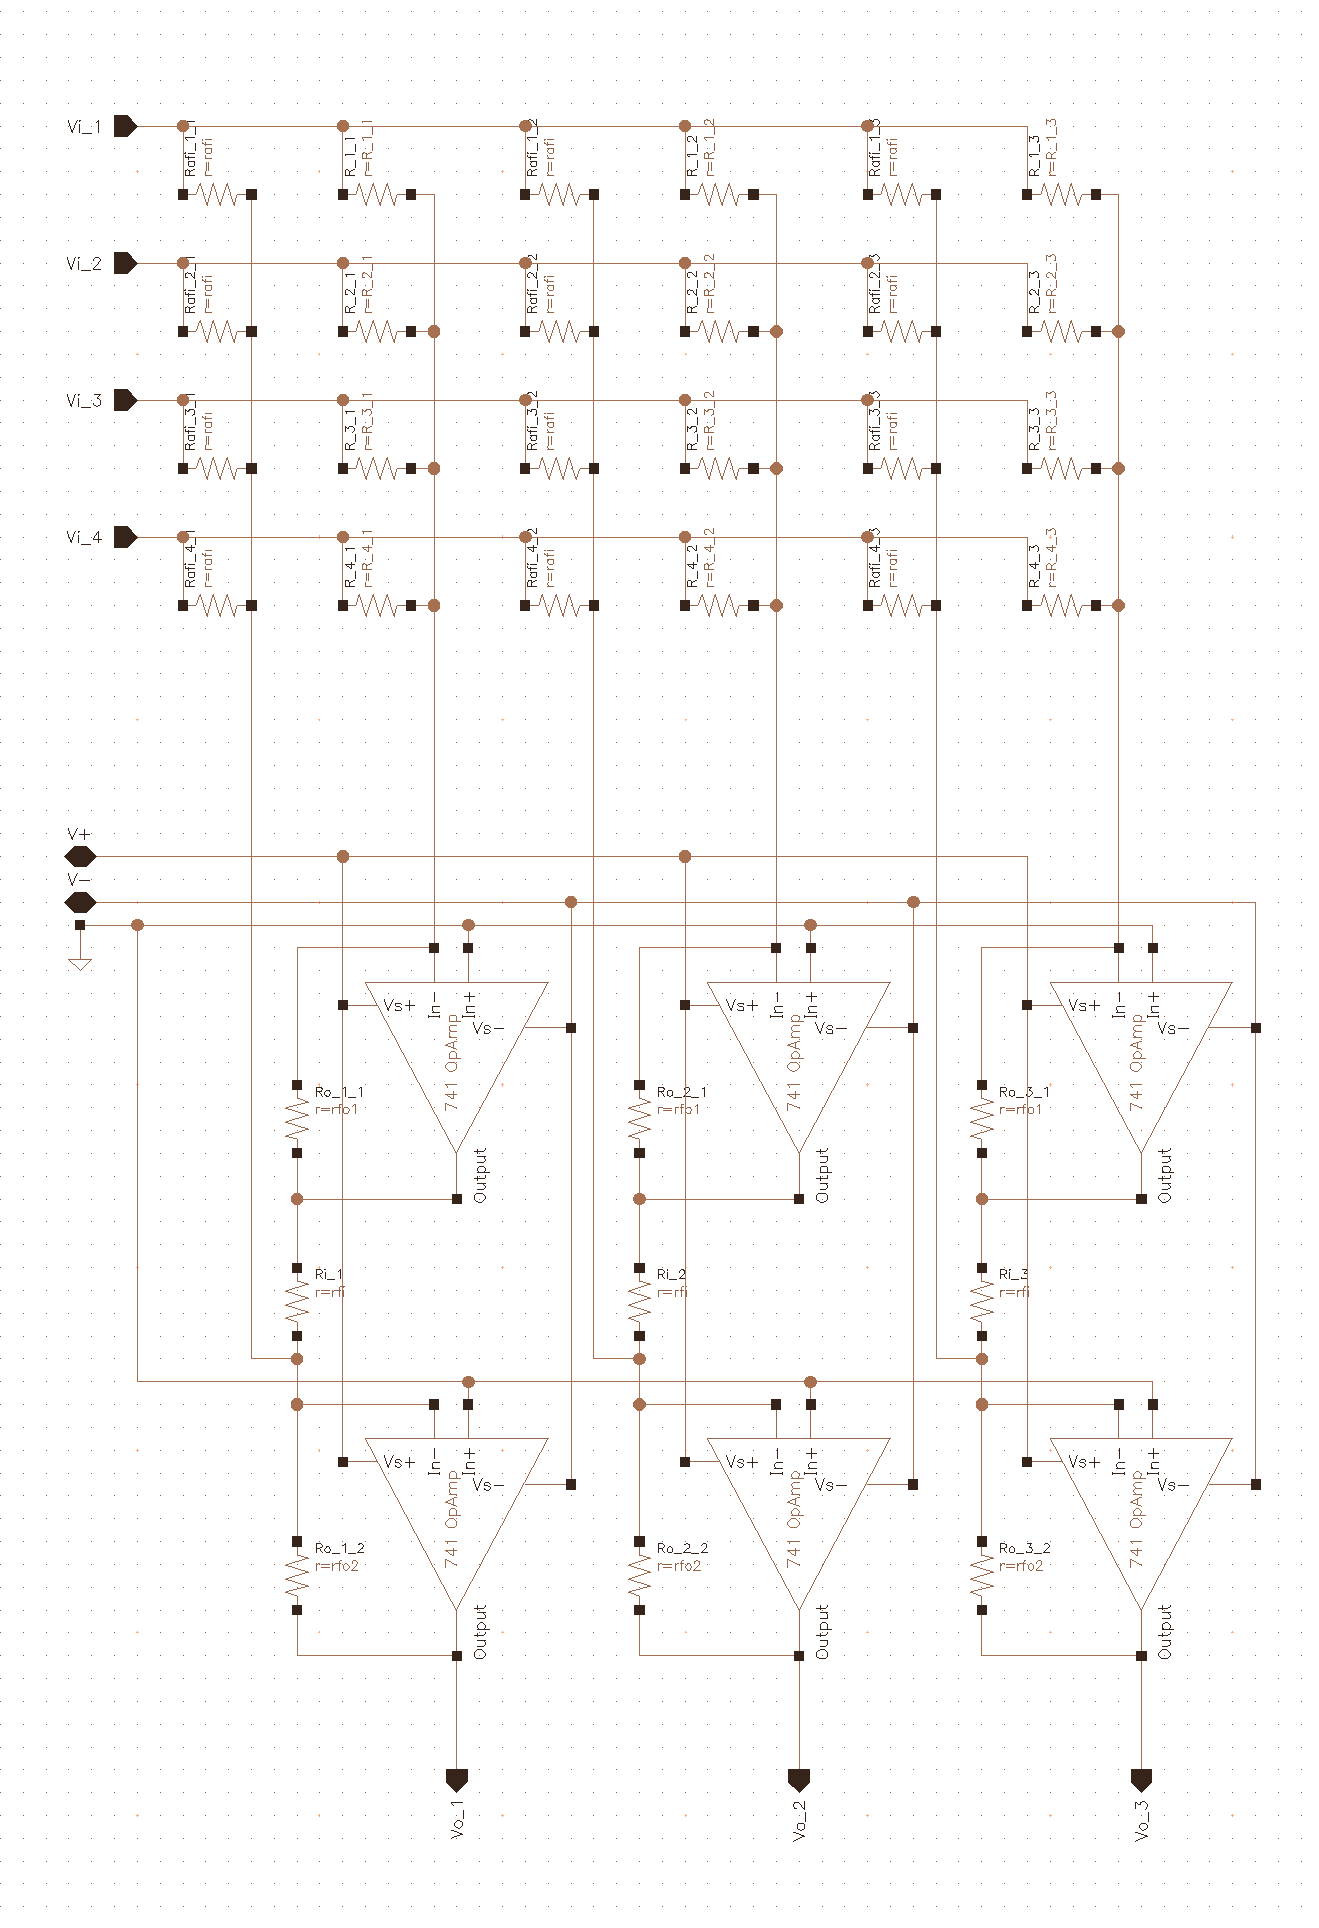
\includegraphics[scale=0.4]{version3.png}
	\caption{4 by 4 generated summing neuron with weight decompression circuit implemented in Cadence}
\end{figure}
\subsubsection{$\text{4}^{\text{th}}$ version} % dual stage
This version design is put forward by co-supervisor due to disappointing performance of very large scale (784 by 20 synapses) implementation of last version. Last version has extremely good performance in closeness in percent relation to ideal, with average scaled up to $100\%$, and error rate ($\text{S.D.} = 2.17\%$) in small scale (20 by 10 synapses) but $\text{S.D.}\approx 54\%$ in large scale.

Therefore, the idea was to break up large scale implementation to an equivalent 2 stage small scale implementation to improve the performance. Interestingly, the idea doesn't work, as we still see $\text{S.D.}\approx 54\%$ in this version too. For more info, see Challenges section.
\begin{figure}[H]
	\centering
	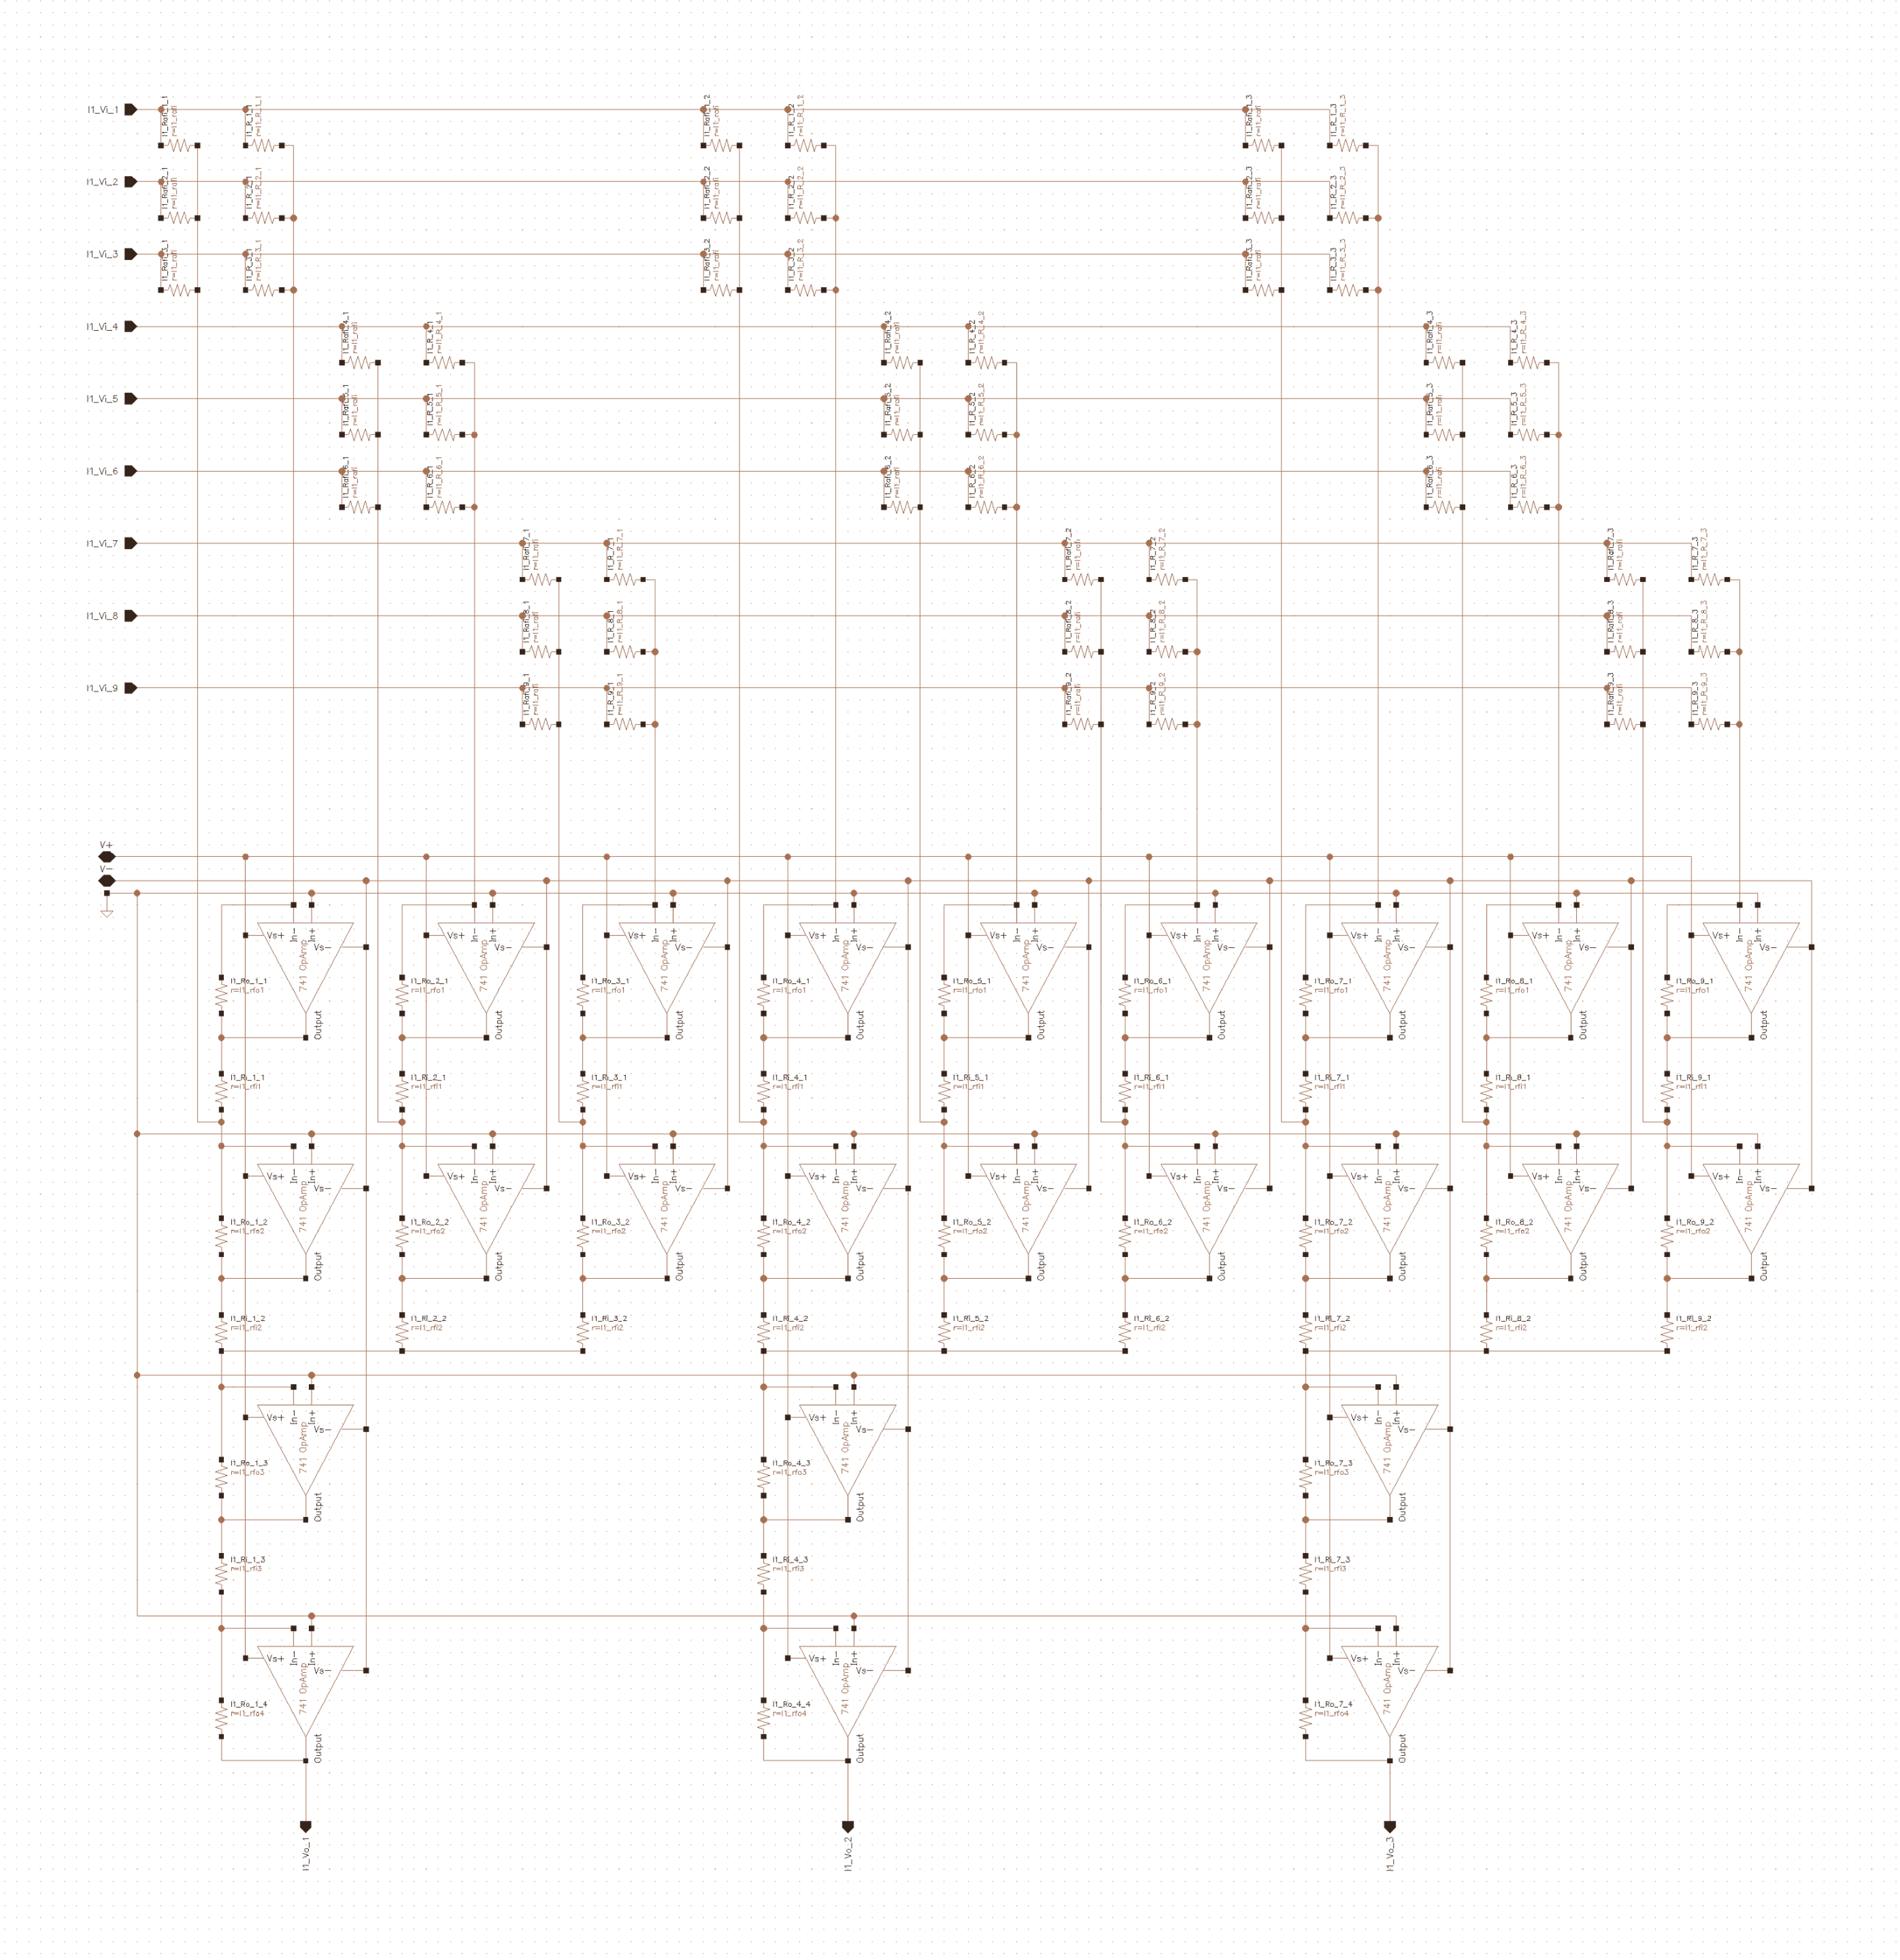
\includegraphics[scale=0.2]{version4.png}
	\caption{9 by 3 dual-stage with 3 in 1st stage and weight decompression circuit generated summing neuron implemented in Cadence}
\end{figure}